\chapter{Fylogenetische bomen en de moleculaire klok}\label{ch:b2:phylogenetic-trees}

In 1965 vergeleken twee chemici, Emile Zuckerkandl en Linus Pauling, de
aminozuursequenties van hemoglobine van een handvol gewervelden en merkten ze
iets op wat geen anatoom had kunnen zien: het aantal verschillen tussen twee
soorten was evenredig met de tijd sinds hun voorouders uiteengingen, zoals
afgelezen uit fossielen. Een molecuul hield de tijd bij. Binnen tien jaar had
Carl Woese één gen, het RNA van de kleine ribosomale subeenheid, gebruikt om de
stamboom van al het leven te tekenen en er een derde domein in te vinden, de
archaea, die geen microscoop van bacteriën had onderscheiden. Dit hoofdstuk
gaat over het reconstrueren van geschiedenis uit gelijkenis: wat een boom
betekent, hoe men er een bouwt uit kenmerken en uit afstanden, hoe men
sequenties de tijd laat vertellen, en de valkuilen --- convergentie, ongelijke
snelheden, verzadiging, lange takken --- die een lezer van bomen moet kennen.

\section{Een boom lezen}

\begin{definition}[Fylogenie, clade, homologie]\label{def:b2:phylogenetic-trees:tree}
\index{fylogenie}\index{clade}\index{monofyletische groep}\index{parafyletische groep}\index{polyfyletische groep}\index{homologie}\index{analogie}\index{synapomorfie}
Een \emph{fylogenie} is een boom waarvan de uiteinden de vergeleken soorten
(of genen, of individuen) zijn, waarvan de inwendige knopen hun gemeenschappelijke
voorouders zijn, en waarvan de wortel de oudste voorouder van allemaal is.
Alleen de vertakkingsvolgorde draagt de geschiedenis: knopen mogen vrij worden
gedraaid, en alleen de nesting telt. Een \emph{clade} of
\emph{monofyletische groep} is een voorouder met \emph{al} zijn
afstammelingen (vogels; zoogdieren; vogels en krokodillen samen);
een \emph{parafyletische} groep is een voorouder waarvan sommige afstammelingen
zijn weggelaten (``reptielen'' zonder vogels, ``vissen'' zonder tetrapoden,
``prokaryoten''); een \emph{polyfyletische} groep verenigt afstammelingen van
verschillende voorouders op grond van een gelijkenis die ze afzonderlijk
ontwikkelden (``warmbloedige dieren''). Een kenmerk dat twee soorten delen
omdat hun voorouder het had, is een \emph{homologie} (de botten van
de vleugel van de vleermuis en de vin van de walvis); een kenmerk dat ze
onafhankelijk ontwikkelden, is een \emph{analogie} of \emph{homoplasie} (de
vleugels van vleermuizen en vogels als vleugels, de cameraogen van gewervelden
en octopussen). Alleen homologieën leggen geschiedenis vast, en onder hen
definiëren alleen de \emph{afgeleide} toestanden die een groep deelt --- haar
\emph{synapomorfieën}, het woord van Hennig --- een clade: veren
definiëren de vogels, de voorouderlijke toestand ``geen veren'' definieert niets.
\end{definition}

\begin{omfigure}
\begin{tikzpicture}[every node/.style={font=\scriptsize}, >=stealth, line width=0.8pt]
  \coordinate (root) at (0,0);
  \coordinate (n1) at (1.2,0.9); \coordinate (n2) at (2.4,1.6); \coordinate (n3) at (3.6,2.3);
  \draw (root) -- (1.4,-1.3) node[right] {zoogdieren};
  \draw (root) -- (n1);
  \draw (n1) -- (4.8,-0.1) node[right] {schildpadden};
  \draw (n1) -- (n2);
  \draw (n2) -- (4.8,0.9) node[right] {hagedissen, slangen};
  \draw (n2) -- (n3);
  \draw (n3) -- (4.8,1.9) node[right] {krokodillen};
  \draw (n3) -- (4.8,3.0) node[right] {vogels};
  \fill (root) circle (1.6pt); \fill (n1) circle (1.6pt); \fill (n2) circle (1.6pt); \fill (n3) circle (1.6pt);
  \node[left] at (root) {amnioten};
  % groups
  \draw[omThm, thick, rounded corners=6pt] (3.1,1.55) rectangle (6.9,3.4);
  \node[omThm, anchor=south west] at (3.1,3.4) {archosauriërs: monofyletisch};
  \draw[omExo!80!black, thick, dashed, rounded corners=6pt] (2.2,-0.5) -- (2.2,2.2) -- (7.1,2.2) -- (7.1,-0.5) -- cycle;
  \node[omExo!80!black, anchor=north east] at (7.1,-0.55) {``reptielen'' zonder vogels: parafyletisch};
  \node[anchor=west, align=left, text width=4.2cm] at (7.9,1.3) {synapomorfieën:\\ $\bullet$ amnionei (alle)\\ $\bullet$ antorbitale opening in de schedel (archosauriërs)\\ $\bullet$ veren (vogels)};
\end{tikzpicture}

{\small Een boom lezen. Vogels zitten genest binnen de reptielen: krokodillen
staan dichter bij vogels dan bij hagedissen. De benoemde groep ``reptielen'' is
een voorouder waarvan één lijn afstammelingen is weggenomen --- een
parafyletische graad, geen \omterm{def:b2:phylogenetic-trees:tree}{clade}.}
\end{omfigure}

\begin{omfigure}
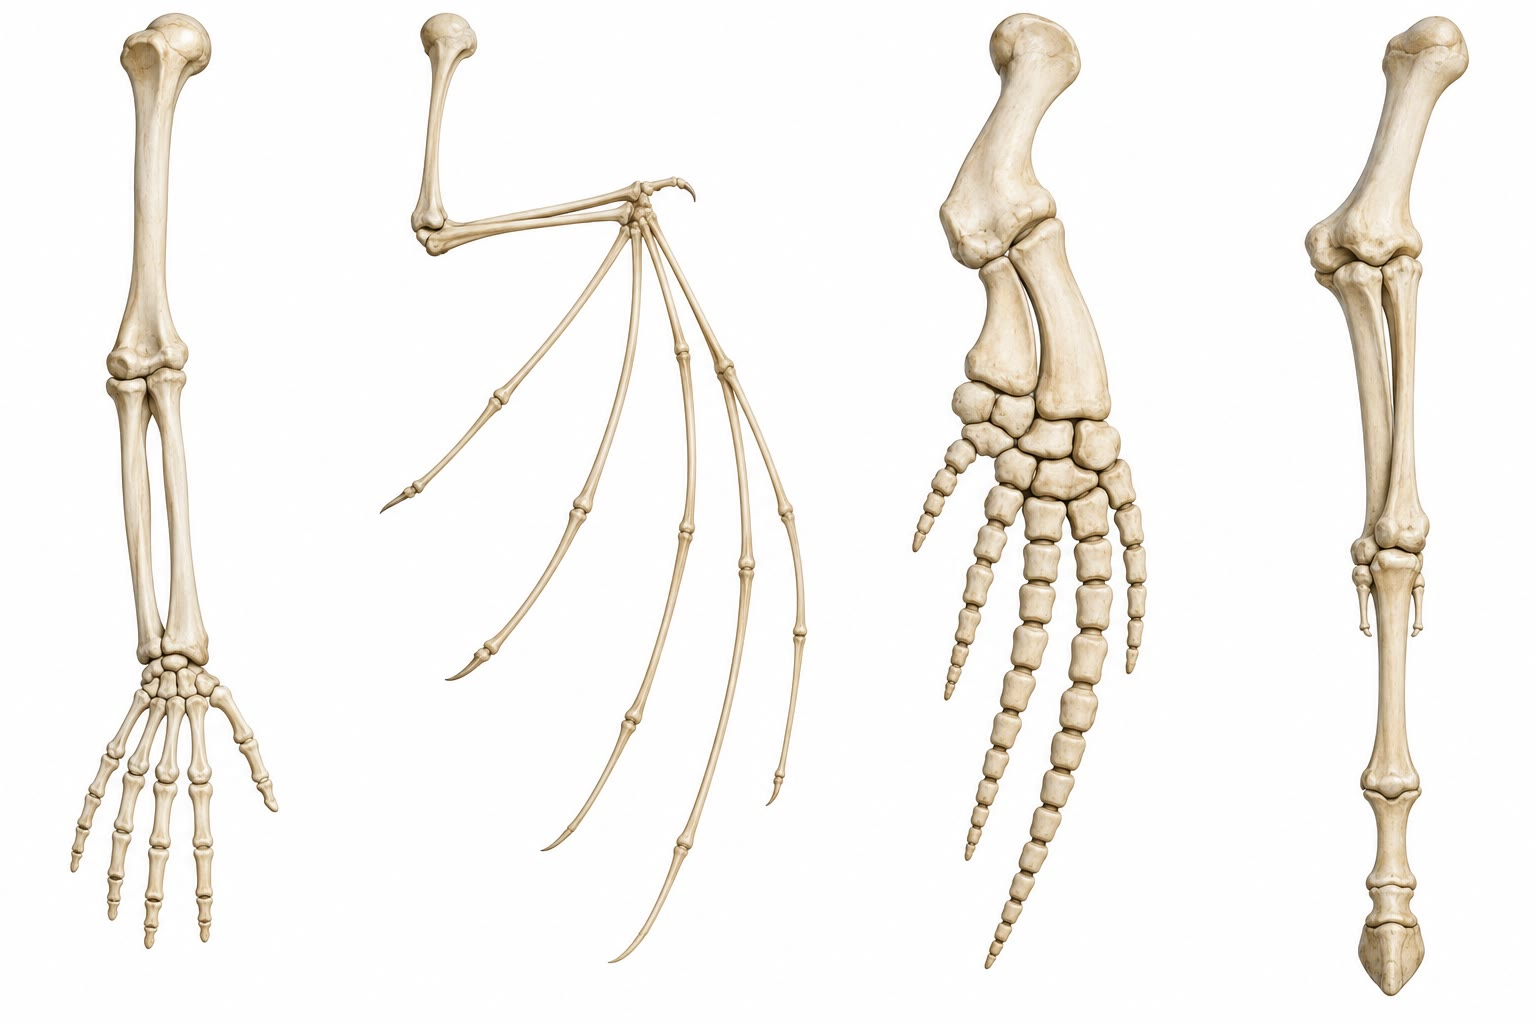
\includegraphics[width=0.44\linewidth]{images/book4/ai/b4-24-homologous-forelimbs.jpg}\hspace{0.04\linewidth}
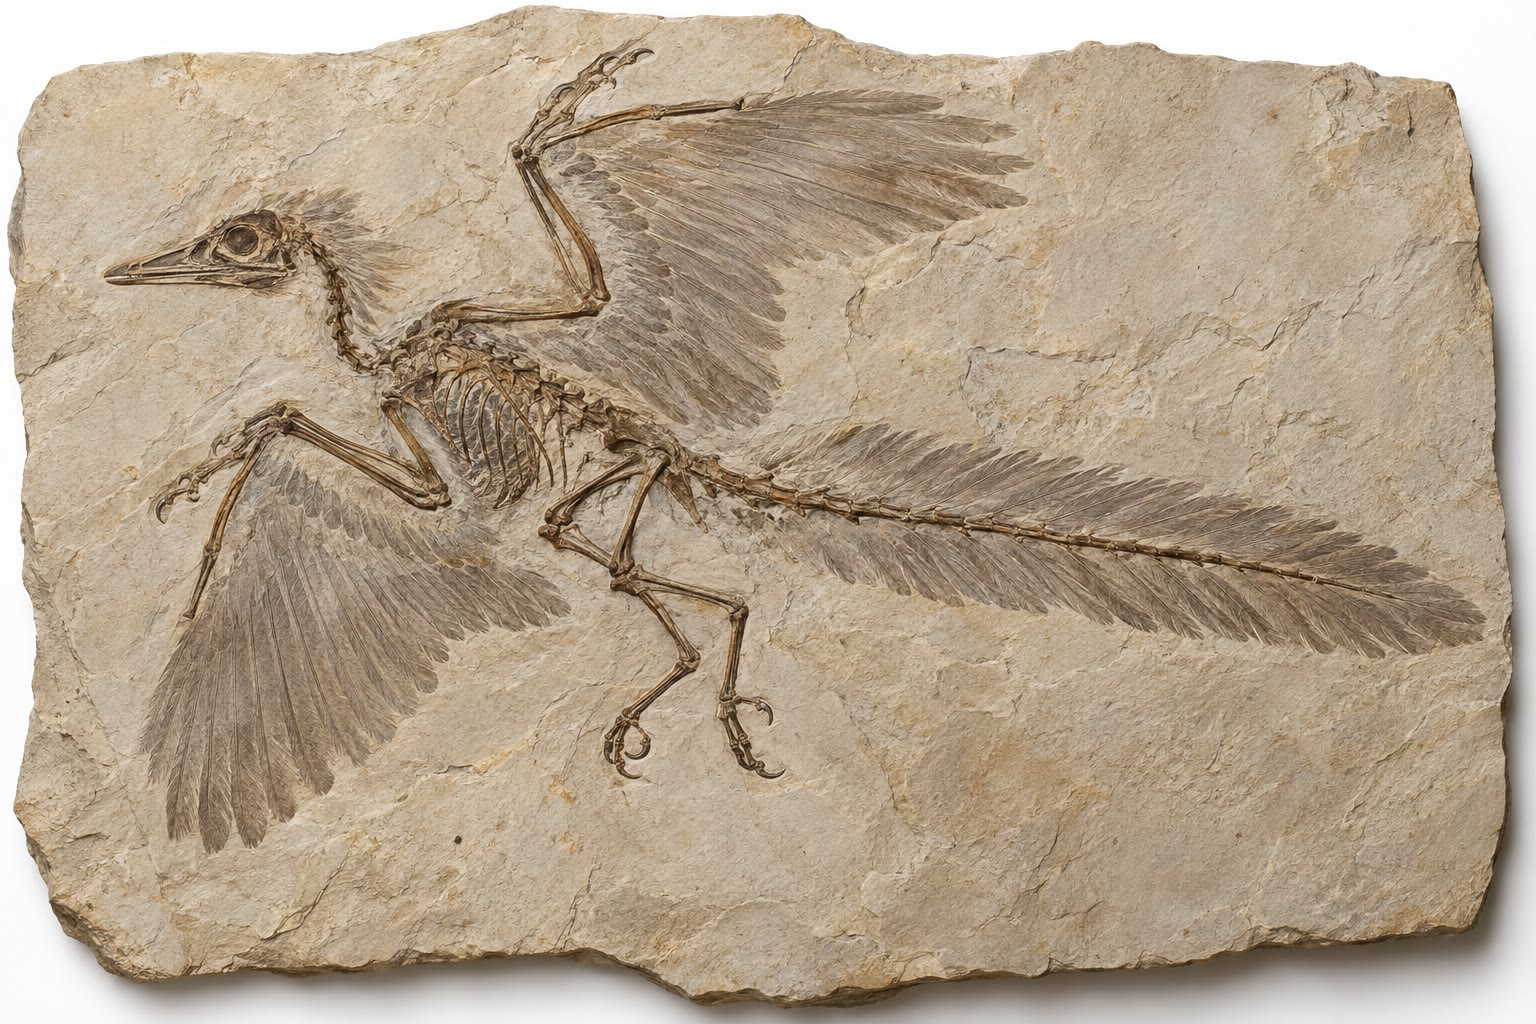
\includegraphics[width=0.44\linewidth]{images/book4/ai/b4-24-archaeopteryx.jpg}

{\small \omterm{def:b2:phylogenetic-trees:tree}{Homologie} en haar vastlegging. Links: dezelfde botten --- opperarmbeen,
spaakbeen en ellepijp, pols, vijf vingers --- in een arm, een vleugel, een vin
en een poot. Rechts: \emph{Archaeopteryx}, met de tanden, geklauwde
vingers en lange benige staart van een kleine dinosauriër en de veren van een
vogel.}
\end{omfigure}

\section{Bomen bouwen uit kenmerken}

\begin{method}[Spaarzaamheid]\label{meth:b2:phylogenetic-trees:parsimony}
\index{spaarzaamheid}\index{buitengroep}\index{bootstrap}
Codeer de kenmerken (morfologische toestanden of gealigneerde
sequentieposities) voor elk taxon. Tel voor elke mogelijke boom het
minimale aantal kenmerkveranderingen dat nodig is om de gegevens erop te
verklaren; de spaarzaamste boom heeft er het minst nodig. Wortel de boom met
een \emph{buitengroep}, een taxon waarvan bekend is dat het buiten de
bestudeerde groep ligt. Omdat het aantal ongewortelde bomen voor $n$ taxa $1\cdot 3\cdot
5\cdots(2n - 5)$ is --- drie voor vier taxa, $2\times 10^{6}$ voor tien,
$10^{20}$ voor twintig --- is de zoektocht alleen voor kleine sets
uitputtend en daarbuiten heuristisch. Het vertrouwen wordt gemeten met de
\emph{bootstrap}: trek de kenmerken duizend keer opnieuw met teruglegging,
bouw de boom telkens opnieuw, en noteer hoe vaak elke \omterm{def:b2:phylogenetic-trees:tree}{clade} terugkomt; een
\omterm{def:b2:phylogenetic-trees:tree}{clade} die in \qty{95}{\%} van de hersteekproeven wordt gevonden, is goed
ondersteund, een die in de helft wordt gevonden niet.
\end{method}

\begin{example}[Vier taxa, vijf posities]\label{ex:b2:phylogenetic-trees:parsimony}
Sequenties $A = \mathrm{AAGCT}$, $B = \mathrm{AAGCC}$, $C =
\mathrm{GGACT}$, $D = \mathrm{GGATC}$. Op de boom $((A,B),(C,D))$
veranderen posities 1, 2 en 3 elk één keer (op de inwendige tak), positie 4
één keer ($\mathrm{C}\to\mathrm{T}$ in $D$) en positie 5 twee keer
($\mathrm{T}\to\mathrm{C}$ in $B$ en in $D$): zes stappen. Op
$((A,C),(B,D))$ vragen posities 1--3 elk twee veranderingen, posities 4 en 5
elk één: acht. Op $((A,D),(B,C))$: negen. De eerste boom is het spaarzaamst,
met twee stappen verschil; de drie posities die hem ondersteunen, zijn
zijn synapomorfieën, en positie 5 is er een homoplasie op --- dezelfde
verandering die twee keer optreedt, een gegeven in elke echte dataset.
\end{example}

\begin{omfigure}
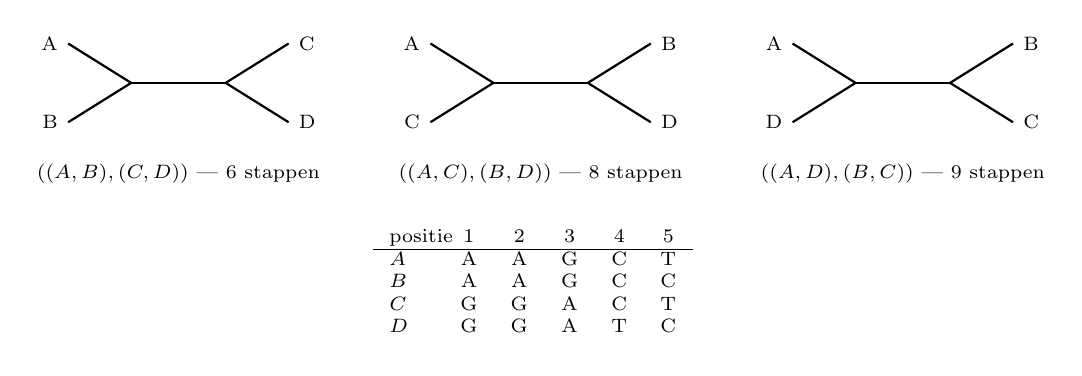
\begin{tikzpicture}[every node/.style={font=\scriptsize}, line width=0.8pt]
  \foreach \x/\a/\b/\c/\d/\steps/\lab in {0/A/B/C/D/6/{$((A,B),(C,D))$ --- 6 stappen}, 4.6/A/C/B/D/8/{$((A,C),(B,D))$ --- 8 stappen}, 9.2/A/D/B/C/9/{$((A,D),(B,C))$ --- 9 stappen}} {
    \begin{scope}[xshift=\x cm]
      \draw (0,1.6) node[left] {\a} -- (0.8,1.1) -- (0,0.6) node[left] {\b};
      \draw (0.8,1.1) -- (2.0,1.1);
      \draw (2.8,1.6) node[right] {\c} -- (2.0,1.1) -- (2.8,0.6) node[right] {\d};
      \node[anchor=north] at (1.4,0.2) {\lab};
    \end{scope}
  }
  \node[anchor=north] at (5.9,-0.6) {\begin{tabular}{l@{\ }ccccc} positie & 1 & 2 & 3 & 4 & 5 \\ \hline $A$ & A & A & G & C & T \\ $B$ & A & A & G & C & C \\ $C$ & G & G & A & C & T \\ $D$ & G & G & A & T & C \end{tabular}};
\end{tikzpicture}

{\small De drie ongewortelde bomen voor vier taxa, gescoord tegen de
alignering van vijf posities eronder. Posities 1--3 veranderen één keer op de
eerste boom en twee keer op de andere; posities 4 en 5 variëren en kunnen niet
beslissen.}
\end{omfigure}

\section{Bomen bouwen uit afstanden}

\begin{method}[Clusteren op afstand: UPGMA]\label{meth:b2:phylogenetic-trees:upgma}
\index{UPGMA}\index{neighbour-joining}\index{afstandsmatrix}
Voeg, uitgaande van de paarsgewijze afstanden tussen $n$ taxa (verschillen per
positie, gecorrigeerd zoals hieronder), het dichtstbijzijnde paar samen tot een
cluster op een knoop met als hoogte de helft van hun afstand; vervang het paar
door de cluster, waarvan de afstand tot elk ander taxon het gemiddelde is van
de afstanden van zijn leden; herhaal tot er één cluster overblijft. Het
resultaat is een gewortelde boom met alle uiteinden op dezelfde hoogte --- het
veronderstelt een constante veranderingssnelheid op elke tak, een \omterm{thm:b2:phylogenetic-trees:clock}{moleculaire
klok}. Wanneer de snelheden tussen lijnen verschillen, groepeert de methode snel
evoluerende lijnen samen, wat hun geschiedenis ook is; \emph{\omterm{ex:b2:phylogenetic-trees:parsimony}{neighbour-joining}},
dat bij elke stap het paar samenvoegt waarvan de vereniging de hele boom het
meest verkort, veronderstelt geen klok en is de gangbare snelle methode
voor grote datasets.
\end{method}

\begin{example}[UPGMA]\label{ex:b2:phylogenetic-trees:upgma}
Afstanden (in verschillen per honderd posities): $AB = 4$, $AC = 8$,
$AD = 10$, $BC = 8$, $BD = 10$, $CD = 6$. Voeg $A$ en $B$ samen op hoogte 2;
dan $d(AB, C) = 8$, $d(AB, D) = 10$, $d(C,D) = 6$: voeg $C$ en $D$ samen op
hoogte 3; ten slotte $d(AB, CD) = (8 + 10 + 8 + 10)/4 = 9$: voeg de
twee clusters samen op hoogte $4.5$. De boom is $((A,B),(C,D))$, en als
de snelheid $10^{-9}$ substituties per positie per jaar is, is de wortel
$0.045/10^{-9} = 45$ miljoen jaar oud.
\end{example}

\begin{omfigure}
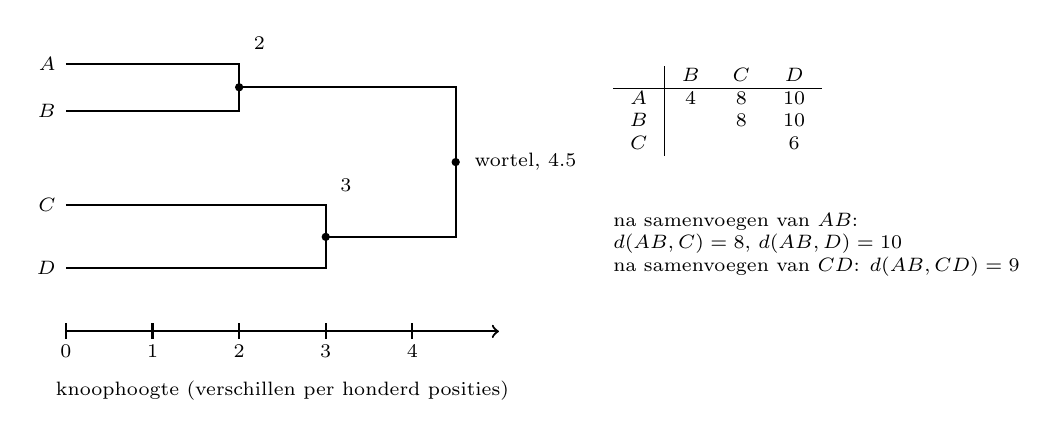
\begin{tikzpicture}[every node/.style={font=\scriptsize}, line width=0.8pt, x=1.1cm]
  \draw[->] (0,-0.4) -- (5,-0.4); \foreach \h in {0,1,2,3,4} \draw (\h,-0.5) -- (\h,-0.3) node[below=4pt] {\h};
  \node[anchor=north] at (2.5,-0.9) {knoophoogte (verschillen per honderd posities)};
  % A,B join at 2, C,D at 3, root at 4.5 ; draw as rooted tree, root on the right
  \draw (0,3.0) node[left] {$A$} -- (2,3.0) -- (2,2.4) -- (0,2.4) node[left] {$B$};
  \draw (0,1.2) node[left] {$C$} -- (3,1.2) -- (3,0.4) -- (0,0.4) node[left] {$D$};
  \draw (2,2.7) -- (4.5,2.7) -- (4.5,0.8) -- (3,0.8);
  \fill (2,2.7) circle (1.5pt); \fill (3,0.8) circle (1.5pt); \fill (4.5,1.75) circle (1.5pt);
  \node[anchor=west] at (4.6,1.75) {wortel, 4.5};
  \node[anchor=south west] at (2.05,3.05) {2};
  \node[anchor=south west] at (3.05,1.25) {3};
  \node[anchor=west, align=left] at (6.2,2.4) {\begin{tabular}{c|ccc} & $B$ & $C$ & $D$ \\ \hline $A$ & 4 & 8 & 10 \\ $B$ & & 8 & 10 \\ $C$ & & & 6 \end{tabular}};
  \node[anchor=west, align=left] at (6.2,0.7) {na samenvoegen van $AB$:\\ $d(AB,C) = 8$, $d(AB,D) = 10$\\ na samenvoegen van $CD$: $d(AB,CD) = 9$};
\end{tikzpicture}

{\small UPGMA op vier taxa. Elke knoop ligt op de helft van de afstand
tussen de clusters die hij samenvoegt; elk uiteinde eindigt op hoogte nul, zoals
een klok vereist.}
\end{omfigure}

\section{De moleculaire klok}

\begin{theorem}[Substituties als poissonproces, en de correctie voor meervoudige treffers]\label{thm:b2:phylogenetic-trees:clock}
\index{moleculaire klok}\index{correctie van Jukes--Cantor}\index{verzadiging}
Als substituties op een positie met een constante snelheid $k$ per jaar
optreden, onafhankelijk over de posities, is het aantal dat zich langs een
lijn in een tijd $t$ opstapelt poissonverdeeld met gemiddelde $kt$, en is het
verwachte aantal dat twee lijnen scheidt die $t$ jaar geleden uiteengingen
\[
d = 2kt
\]
substituties per positie --- de \emph{\omterm{thm:b2:phylogenetic-trees:clock}{moleculaire klok}}. De waargenomen
fractie $p$ van verschillende posities is kleiner dan $d$, omdat een
positie die twee keer wordt getroffen naar haar oorspronkelijke base kan
terugkeren of toevallig overeenkomen; met vier basen die met gelijke snelheden
veranderen, geldt
\[
p = \tfrac{3}{4}\bigl(1 - e^{-4d/3}\bigr), \qquad
d = -\tfrac{3}{4}\ln\bigl(1 - \tfrac{4}{3}p\bigr),
\]
de correctie van \emph{Jukes--Cantor}. Naarmate $d$ groeit, verzadigt $p$ op
$3/4$ --- twee willekeurige sequenties komen op een kwart van hun posities
overeen --- en voorbij $p \approx 0.5$ vergroot de correctie elke
steekproeffout: een gen dat zoveel veranderd is, houdt de tijd niet meer bij.
Trage genen (ribosomaal RNA, histonen) dateren de diepe takken, snelle
(mitochondriaal DNA, introns) de recente.
\end{theorem}
\begin{proof}
Zij $q(t)$ de kans dat een positie na een tijd $t$ nog haar oorspronkelijke
base draagt. Die gaat verloren met snelheid $k$ en wordt, vanuit elk van de
drie andere basen, teruggewonnen met snelheid $k/3$:
$\mathrm{d}q/\mathrm{d}t = -kq + \tfrac{k}{3}(1 - q) = \tfrac{k}{3} -
\tfrac{4k}{3}q$, met als oplossing bij $q(0) = 1$ $q = \tfrac14 +
\tfrac34 e^{-4kt/3}$. Twee lijnen gescheiden door een totale tijd $2t$ ---
door symmetrie hetzelfde als één lijn die $2t$ lang evolueert --- komen op
een positie overeen met kans $\tfrac14 + \tfrac34 e^{-4d/3}$, waarin $d =
2kt$, dus $p = 1 - q = \tfrac34(1 - e^{-4d/3})$; omkeren geeft de
correctie. De poissontelling volgt uit constante, onafhankelijke
gebeurtenissen, zoals in de natuurkunde van radioactief verval, en haar
standaardafwijking $\sqrt{kt}$ bepaalt de nauwkeurigheid van elke datering: een
gen van $L$ posities met $dL$ waargenomen substituties dateert een
divergentie met een relatieve nauwkeurigheid van ongeveer $1/\sqrt{dL}$.
\end{proof}
\begin{proof}[Bewijsmateriaal]
Zuckerkandl en Pauling (1965) vonden dat de verschillen tussen de hemoglobinen
van paard, mens, rund en andere soorten evenredig waren met de fossiele
ouderdom van hun splitsingen, en stelden de klok voor. Fitch en
Margoliash (1967) bouwden alleen uit cytochroom
$c$ een boom van twintig soorten en vonden, uit één enkel eiwit, de klassieke
groeperingen van gewervelden, insecten en schimmels terug. De beslissende test
van de methode was de experimentele \omterm{def:b2:phylogenetic-trees:tree}{fylogenie} van Hillis en collega's (1992):
ze lieten bacteriofaag T7 onder een mutageen een bekende, vertakkende reeks van
acht lijnen doorlopen, sequeneerden de producten, en gaven de sequenties blind
aan de methoden om bomen te bouwen --- spaarzaamheids-, afstands- en
likelihoodmethoden vonden allemaal de ware boom terug, en spaarzaamheid
reconstrueerde de voorouderlijke sequenties met een nauwkeurigheid van meer dan
\qty{98}{\%}.
\end{proof}

\begin{omfigure}
\begin{tikzpicture}
\begin{axis}[
  width=0.7\linewidth, height=5.4cm,
  axis x line=bottom, axis y line=left,
  xmin=0, xmax=2.5, ymin=0, ymax=1.05,
  xlabel={ware substituties per positie, $d$}, ylabel={waargenomen verschillen, $p$},
  xlabel style={font=\small, at={(axis description cs:0.5,-0.13)}, anchor=north},
  ylabel style={font=\small},
  tick label style={font=\small}, ytick={0,0.25,0.5,0.75,1},
  legend style={font=\scriptsize, at={(0.97,0.35)}, anchor=east, draw=none},
  clip=false,
]
\addplot[very thick, omDef, domain=0:2.5, samples=80] {0.75*(1-exp(-4*x/3))};
\addlegendentry{$p = \tfrac34(1 - e^{-4d/3})$}
\addplot[thick, gray, dashed, domain=0:1.05, samples=2] {x};
\addlegendentry{$p = d$: geen meervoudige treffers}
\draw[dotted, gray] (axis cs:0,0.75) -- (axis cs:2.5,0.75); \node[font=\scriptsize, anchor=south east] at (axis cs:2.5,0.75) {verzadiging, $p = 3/4$};
\draw[<->, omThm, thick] (axis cs:0.383,0.30) -- (axis cs:0.383,0.383); \node[font=\scriptsize, omThm, anchor=west] at (axis cs:0.5,0.22) {$p = 0.30$ betekent $d = 0.38$};
\end{axis}
\end{tikzpicture}

{\small Meervoudige treffers. De waargenomen fractie verschillende posities
stijgt met het ware aantal substituties en verzadigt dan; een ruwe $p$
onderschat elke afstand en drukt de diepe takken van een boom in elkaar.}
\end{omfigure}

\begin{proposition}[Valkuilen van de klok en van bomen]\label{prop:b2:phylogenetic-trees:pitfalls}
\index{aantrekking van lange takken}\index{snelheidsheterogeniteit}\index{onvolledige lijnsortering}\index{likelihood (fylogenetica)}
De klok is maar bij benadering constant: de snelheden verschillen tussen
genen met een factor honderd (naargelang de functie --- histon H4 heeft in een
miljard jaar twee residuen veranderd, fibrinopeptiden veranderen om de paar
miljoen jaar), tussen posities binnen een gen (derde codonposities, introns en
lussen veranderen het snelst), en tussen lijnen (knaagdieren tikken sneller
dan primaten, met hun kortere generaties en hogere stofwisseling). Elke
klok heeft dus \emph{kalibratie} nodig met een fossiel of een gedateerde
geologische gebeurtenis, en dateringen dragen de poissonfout hierboven en die
van de kalibratie zelf. Bomen hebben hun eigen valkuilen. \emph{\omterm{prop:b2:phylogenetic-trees:pitfalls}{Aantrekking van
lange takken}}: twee lijnen die elk sterk veranderd zijn, delen toevallig veel
posities, en spaarzaamheid voegt ze samen wat hun geschiedenis ook is --- de
remedie is een dichtere bemonstering om de takken te onderbreken en een
methode die de snelheden modelleert. \emph{Convergentie} levert valse
synapomorfieën op. \emph{\omterm{prop:b2:phylogenetic-trees:pitfalls}{Onvolledige lijnsortering}}: de boom van een gen hoeft
niet de boom van de soorten te zijn wanneer soortvormingen snel op elkaar
volgen, omdat het voorouderlijke polymorfisme zich in elke afstammeling anders
sorteert --- en daarom wordt een soortenboom uit veel genen gebouwd, niet uit
één. En bij prokaryoten, waar genen zijdelings bewegen
(\cref{ch:b2:genome-diversification}), vertellen verschillende genen
verschillende verhalen en is de geschiedenis een web waar een boom van
ribosomale genen doorheen loopt. De moderne praktijk vervangt spaarzaamheid en
afstand door \emph{likelihood}: bereken, gegeven een substitutiemodel (de
snelheden van elke verandering, hun variatie tussen posities), de kans op de
waargenomen sequenties op elke boom met zijn taklengtes, en kies de boom die de
gegevens het waarschijnlijkst maakt; de bayesiaanse vorm ervan levert
rechtstreeks een kans voor elke \omterm{def:b2:phylogenetic-trees:tree}{clade} op.
Het deel van jaar 3 geeft de methoden; hier volstaat het te weten dat
elke boom een hypothese is met een gemeten ondersteuning, geen feit.
\end{proposition}
\begin{proof}[Bewijsmateriaal]
Woese en Fox (1977) vergeleken het ribosomale RNA van de kleine subeenheid bij
prokaryoten en vonden de methanogenen even ver van de bacteriën als elk van
beide van de eukaryoten: de drie domeinen, sindsdien bevestigd door elk gen van
de transcriptie- en translatiemachinerie, en onzichtbaar voor de morfologie.
Dezelfde ribosomale bomen, naïef gelezen, plaatsten de snel evoluerende
microsporidiën aan de basis van de eukaryoten; genen met tragere snelheden, en
modellen die snelheidsvariatie toelaten, verplaatsten ze naar de schimmels,
waar ze thuishoren --- een schoolvoorbeeld van \omterm{prop:b2:phylogenetic-trees:pitfalls}{aantrekking van lange takken},
opgespoord en verholpen.
\end{proof}

\begin{omfigure}
\begin{tikzpicture}[every node/.style={font=\scriptsize}, line width=0.8pt]
  \node[anchor=south] at (1.5,2.6) {ware boom};
  \draw (0,2.2) node[left] {$A$} -- (0.8,1.6) -- (0,1.0) node[left] {$B$};
  \draw (0.8,1.6) -- (1.6,1.6);
  \draw[very thick, omThm] (1.6,1.6) -- (3.4,2.4) node[right] {$C$ (snel)};
  \draw[very thick, omThm] (0.8,1.6) -- (0.8,0.2) -- (2.6,0.2) node[right] {$D$ (snel)};
  \draw (1.6,1.6) -- (2.4,1.0) node[right] {$E$};
  \begin{scope}[xshift=7cm]
    \node[anchor=south] at (1.5,2.6) {boom volgens spaarzaamheid};
    \draw (0,2.2) node[left] {$A$} -- (0.8,1.6) -- (0,1.0) node[left] {$B$};
    \draw (0.8,1.6) -- (1.6,1.6);
    \draw (1.6,1.6) -- (2.4,1.9) node[right] {$E$};
    \draw[very thick, omThm] (1.6,1.6) -- (2.2,1.0) -- (3.4,1.3) node[right] {$C$};
    \draw[very thick, omThm] (2.2,1.0) -- (3.0,0.2) node[right] {$D$};
  \end{scope}
  \node[align=center, text width=7cm] at (5.6,-1.1) {$C$ en $D$ zijn elk op veel posities veranderd; op een kwart daarvan komen ze nu toevallig overeen, meer dan enige ware synapomorfie ze met hun echte verwanten verbindt};
\end{tikzpicture}

{\small \omterm{prop:b2:phylogenetic-trees:pitfalls}{Aantrekking van lange takken}. Twee lijnen die het snelst zijn
geëvolueerd, worden samengevoegd door de toevallige overeenkomsten die hun vele
veranderingen opleveren, en spaarzaamheid maakt ze tot zustergroepen.}
\end{omfigure}

\begin{example}[Dateren met een fossiel]\label{ex:b2:phylogenetic-trees:dating}
Een gen van \num{1000} posities verschilt op \qty{10}{\%} ervan tussen
rund en walvis, waarvan de fossielen de gemeenschappelijke voorouder op 60
miljoen jaar plaatsen. Gecorrigeerd is $d = -0.75\ln(1 - 0.133) = 0.107$; de
snelheid is $k
= d/2t = 0.107/(1.2\times 10^{8}) = 9\times 10^{-10}$ per positie per
jaar. Hetzelfde gen verschilt op \qty{6}{\%} tussen walvis en nijlpaard:
$d = 0.0625$, $t = d/2k = 35$ miljoen jaar, met ongeveer $\pm
\qty{13}{\%}$ door de poissontelling van 62 substituties en een
bijkomende onzekerheid door de fossiele datering. Het moleculaire resultaat
dat walvissen de naaste levende verwanten van de nijlpaarden zijn, in de jaren
1990 zo verkregen tegen elke anatomische boom in, werd bevestigd door de
ontdekking van vroege walvissen met het voorspelde nijlpaardachtige
enkelbot --- de klok dateert niet alleen; ze voorspelt wat de gesteenten
moeten bevatten.
\end{example}

\section{Opgaven}

\begin{exercise}[$\star$]\label{exo:b2:phylogenetic-trees:1}
Definieer \omterm{def:b2:phylogenetic-trees:tree}{homologie}, \omterm{def:b2:phylogenetic-trees:tree}{analogie} en \omterm{def:b2:phylogenetic-trees:tree}{synapomorfie}, met van elk één voorbeeld
uit de ledematen, vleugels en ogen van gewervelden.
\end{exercise}

\begin{exercise}[$\star$]\label{exo:b2:phylogenetic-trees:2}
Deel in als monofyletisch, parafyletisch of polyfyletisch: vogels;
reptielen (zonder vogels); vissen (zonder tetrapoden); vliegende
gewervelden; zoogdieren; prokaryoten.
\end{exercise}

\begin{exercise}[$\star$]\label{exo:b2:phylogenetic-trees:3}
Noem op de boom $(\text{zoogdier},(\text{schildpad},(\text{hagedis},
(\text{krokodil},\text{vogel}))))$ de zustergroep van de
vogels, de zustergroep van de zoogdieren, en de kleinste \omterm{def:b2:phylogenetic-trees:tree}{clade} die
hagedissen en vogels bevat. Verandert het verwisselen van de posities van
krokodillen en vogels de boom?
\end{exercise}

\begin{exercise}[$\star$]\label{exo:b2:phylogenetic-trees:4}
Hoeveel ongewortelde bomen zijn er voor 4, 6 en 10 taxa? Hoeveel
gewortelde bomen voor 4 (elke ongewortelde boom kan op elk van zijn
takken worden geworteld)?
\end{exercise}

\begin{exercise}[$\star\star$]\label{exo:b2:phylogenetic-trees:5}
Sequenties $A = \mathrm{CCTAG}$, $B = \mathrm{CCTGG}$, $C =
\mathrm{TTCAG}$, $D = \mathrm{TTCGA}$. Tel de stappen op elk van de
drie ongewortelde bomen en geef de spaarzaamste. Welke
posities zijn er homoplastisch op?
\end{exercise}

\begin{exercise}[$\star\star$]\label{exo:b2:phylogenetic-trees:6}
Afstanden (per honderd posities): $AB = 6$, $AC = 14$, $AD = 16$,
$BC = 14$, $BD = 16$, $CD = 10$. Bouw de UPGMA-boom met zijn
knoophoogtes.
\end{exercise}

\begin{exercise}[$\star\star$]\label{exo:b2:phylogenetic-trees:7}
Corrigeer $p = 0.05$, $0.30$ en $0.60$ voor meervoudige treffers. Waarom is de
derde waarde bijna nutteloos?
\end{exercise}

\begin{exercise}[$\star\star$]\label{exo:b2:phylogenetic-trees:8}
Een gen evolueert met $10^{-9}$ substituties per positie per jaar. Twee
soorten verschillen met $d = 0.02$: wanneer splitsten ze? Welke $p$ zou
men waarnemen tussen twee soorten die 500 miljoen jaar geleden splitsten,
en wat betekent dat voor het dateren van diepe splitsingen met dit gen?
\end{exercise}

\begin{exercise}[$\star\star$]\label{exo:b2:phylogenetic-trees:9}
Een \omterm{def:b2:phylogenetic-trees:tree}{clade} verschijnt in \qty{52}{\%} van \num{1000} bootstrapsteekproeven;
een andere in \qty{99}{\%}. Interpreteer beide. Wat zou men aan de
eerste doen?
\end{exercise}

\begin{exercise}[$\star\star\star$]\label{exo:b2:phylogenetic-trees:10}
Leg de \omterm{prop:b2:phylogenetic-trees:pitfalls}{aantrekking van lange takken} uit met het argument van het kwart door
toeval, en zeg waarom het toevoegen van taxa die de lange takken onderbreken helpt.
\end{exercise}

\begin{exercise}[$\star\star\star$]\label{exo:b2:phylogenetic-trees:11}
Mitochondriaal DNA van mens en chimpansee verschilt op \qty{9}{\%} van de
posities; de mitochondriale snelheid is ongeveer $2\times 10^{-8}$ per positie
per jaar. Dateer de splitsing, geef de poissononzekerheid voor een
genoom van \qty{16000}{} posities, en noem twee redenen waarom het antwoord
toch een factor twee fout zou kunnen zijn.
\end{exercise}

\begin{exercise}[$\star\star\star$]\label{exo:b2:phylogenetic-trees:12}
``Een genenboom is geen soortenboom.'' Bespreek dit met \omterm{prop:b2:phylogenetic-trees:pitfalls}{onvolledige
lijnsortering}, horizontale overdracht en genduplicatie, en zeg
hoe men toch een soortenboom verkrijgt.
\end{exercise}

\section{Vraagstuk: de walvissen dateren}

\begin{problem}[{Weekendvraagstuk --- walvis, nijlpaard, rund, varken en
kameel gesequeneerd voor één gen: de boom gebouwd met spaarzaamheid en met
afstanden, de klok gekalibreerd op een fossiel, elke splitsing gedateerd met
haar poissonfout, en de anatomische boom geconfronteerd met de
moleculaire, met als besluit de divergentietijd van walvis en nijlpaard en de
substitutiesnelheid van het gen}]
\label{pb:b2:phylogenetic-trees:1}
Een gen van \num{1000} posities wordt gesequeneerd bij walvis ($W$), nijlpaard
($H$), rund ($C$), varken ($P$) en kameel ($M$, de buitengroep). Waargenomen
fracties verschillende posities: $WH = 0.06$; $WC = HC = 0.10$; $WP =
HP = CP = 0.12$; elke afstand tot $M$ is $0.14$. Fossielen plaatsen de
splitsing tussen rund en de lijn van walvis en nijlpaard op 60 miljoen jaar.
Zes informatieve posities, met de toestand van de kameel als laatste:
\begin{center}
\begin{tabular}{l@{\quad}cccccc}
positie & 1 & 2 & 3 & 4 & 5 & 6 \\ \hline
$W$ & A & G & T & C & A & G \\
$H$ & A & G & T & C & G & G \\
$C$ & G & A & T & T & G & G \\
$P$ & G & A & C & T & G & A \\
$M$ & G & A & C & T & G & A \\
\end{tabular}
\end{center}

\medskip
\noindent\textbf{Deel I --- Spaarzaamheid.}
\begin{enumerate}
  \item Welke posities zijn synapomorfieën van $\{W, H\}$? Van $\{W, H,
        C\}$? Welke positie is niet informatief, en welke is een homoplasie
        of autapomorfie?
  \item Tel de stappen van de zes posities op de boom
        $(M,(P,(C,(W,H))))$.
  \item Tel ze op de boom van de anatomen $(M,(P,(W,(C,H))))$,
        die het nijlpaard bij het rund onder de evenhoevigen plaatst en
        de walvissen erbuiten.
  \item Welke boom heeft de voorkeur, en met hoeveel stappen? Waarom is die
        marge zwak, en wat zou haar versterken?
  \item De bootstrap geeft de \omterm{def:b2:phylogenetic-trees:tree}{clade} $\{W, H\}$ in \qty{83}{\%} van de
        hersteekproeven van het hele gen. Interpreteer.
  \item Waarom wordt de kameel als buitengroep gebruikt, en wat zou er
        misgaan als in plaats daarvan een vis werd gebruikt?
\end{enumerate}

\medskip
\noindent\textbf{Deel II --- Afstanden.}
\begin{enumerate}[resume]
  \item Corrigeer de vier verschillende waarden van $p$ ($0.06$, $0.10$, $0.12$,
        $0.14$) voor meervoudige treffers.
  \item Pas UPGMA toe op de vijf taxa met de gecorrigeerde afstanden en
        geef de knoophoogtes.
  \item Stemt de afstandsboom overeen met de spaarzaamheidsboom?
  \item Leg uit waarom UPGMA zou falen als de walvislijn twee keer zo snel
        was geëvolueerd als de andere.
  \item Bereken het aantal substituties dat het gen tussen walvis en
        nijlpaard heeft opgestapeld, en de standaardafwijking ervan volgens
        Poisson.
  \item Geef de relatieve nauwkeurigheid van een datering op basis van dat aantal.
\end{enumerate}

\medskip
\noindent\textbf{Deel III --- De klok.}
\begin{enumerate}[resume]
  \item Kalibreer: bereken uit de afstand tussen rund en (walvis, nijlpaard) en
        het fossiel van 60 miljoen jaar de snelheid $k$ per positie per
        jaar.
  \item Dateer de splitsing tussen walvis en nijlpaard.
  \item Dateer de splitsing van het varken en die van de kameel.
  \item Geef de datering van walvis en nijlpaard met haar poissononzekerheid.
  \item De fossiele kalibratie is zelf onzeker met $\pm 5$
        miljoen jaar. Plant die voort naar de datering van walvis en nijlpaard.
  \item Een ander, sneller gen geeft $p = 0.45$ tussen walvis en
        kameel. Corrigeer dit en geef commentaar op de betrouwbaarheid ervan
        voor deze splitsing.
\end{enumerate}

\medskip
\noindent\textbf{Deel IV --- Confrontatie.}
\begin{enumerate}[resume]
  \item De boom van de anatomen steunt op het enkelbot met dubbele katrol dat
        rund, varken, nijlpaard en kameel delen, maar levende walvissen niet,
        omdat die geen achterpoten hebben. Leg uit waarom een verloren
        kenmerk niet tegen de \omterm{def:b2:phylogenetic-trees:tree}{clade} van walvis en nijlpaard kan pleiten.
  \item In 2001 werden fossiele walvissen met achterpoten gevonden; hun
        enkelbot heeft de dubbele katrol. Wat doet dat met het
        argument?
  \item Als walvissen binnen de evenhoevigen vallen, is de groep
        ``evenhoevigen zonder walvissen'' dan monofyletisch,
        parafyletisch of polyfyletisch?
  \item Een tweede gen geeft de boom $(M,(P,(H,(W,C))))$. Noem twee
        redenen waarom een genenboom kan verschillen van de soortenboom, en
        zeg hoe men beslist.
  \item Het mitochondriale genoom van walvis en nijlpaard verschilt op
        \qty{25}{\%} van de posities. Corrigeer dit, en schat de
        mitochondriale snelheid uit de datering van vraag 14.
  \item Waarom is die snelheid zoveel hoger dan die van het kerngen?
  \item Formuleer het resultaat: de boom, de nucleaire snelheid $k$, en de
        divergentietijd van walvis en nijlpaard met haar onzekerheid.
\end{enumerate}
\end{problem}
